\documentclass{article}

\usepackage[preprint]{neurips_2024}

\usepackage[utf8]{inputenc}
\usepackage[T1]{fontenc}
\usepackage{hyperref}
\usepackage{url}
\usepackage{booktabs}
\usepackage{amsfonts}
\usepackage{amsmath}
\usepackage{nicefrac}
\usepackage{microtype}
\usepackage{xcolor}
\usepackage{graphicx}
\usepackage{subcaption}
\usepackage{multirow}

\title{When Simple Wins:\\Lightweight CNN Encoders for Resource-Constrained Nucleus Segmentation}

\author{
  Danny Rollo \\
  Khoury College of Computer Sciences\\
  Northeastern University\\
  \texttt{rollo.l@northeastern.edu}
}

\begin{document}
\maketitle

\begin{abstract}
For nucleus segmentation pipelines built without large annotated datasets or high-memory GPU infrastructure, a simple VGG U-Net encoder matches purpose-built transformer alternatives at a fraction of the parameter count. We present a controlled comparison of VGG-style, ResNet-style, and Swin Transformer encoders within a shared U-Net framework, evaluated on PanNuke (${\sim}$5K training patches, 19 tissue types) and MoNuSeg (37 training whole-slide images). On PanNuke, VGG (Dice~0.851) matches ResNet (0.849) within single-seed noise and outperforms pretrained Swin by 4.9~Dice points (0.802). On MoNuSeg, VGG (0.796) reaches published MedT-level performance---a transformer designed specifically for small medical datasets---while outperforming pretrained Swin by 4.6~Dice points (0.750). For the deployment scenarios motivating this work---edge-deployed microscopy, veterinary and rare-disease research, and non-H\&E staining protocols where foundation model pretraining misaligns---lightweight from-scratch architectures remain the practical choice, and our results indicate a simple VGG encoder is the strongest option in that design space.
\end{abstract}

%% ============================================================================
\section{Introduction}
%% ============================================================================

Nucleus segmentation in histopathology images underlies a broad range of clinical and research workflows, from tumor microenvironment quantification to cell-cycle analysis. The dominant trend in computational pathology---scaling transformer-based foundation models to hundreds of millions of parameters pretrained on millions of whole-slide images~\cite{chen2024uni, vorontsov2024virchow}---addresses the challenge of limited labeled data but introduces new constraints on deployment.

Recent work has documented practical limits of this approach: foundation models are typically restricted to linear probing rather than full fine-tuning due to memory and stability constraints~\cite{tizhoosh2025why, campanella2025clinical}; their robustness to cross-site distribution shift has been questioned~\cite{dejong2025current}; and their H\&E-pretrained features transfer poorly to non-standard stains such as IHC~\cite{hua2024pathoduet}. For deployment scenarios such as edge-deployed microscopy in under-served clinical settings~\cite{salido2025realtime}, mobile diagnostic platforms, and veterinary or rare-disease research~\cite{xiao2025review} where annotation budgets permit only tens of whole-slide images, lightweight from-scratch architectures remain the practical choice.

This creates a concrete design question: within the space of lightweight, from-scratch architectures, which encoder provides the best performance in the low-data regime? We address this through a controlled ablation using a U-Net with a fixed decoder and shared encoder interface, where the encoder backbone is the only variable. We compare three encoders---VGG-style, ResNet-style, and Swin Transformer---across PanNuke and the genuinely small-data MoNuSeg (37 training images), and show that a VGG encoder outperforms both ResNet and pretrained Swin on PanNuke and matches MedT---a transformer designed specifically for small medical datasets---while outperforming pretrained Swin on MoNuSeg.

\textbf{Contributions.} Our contributions are: (1)~a controlled encoder-family ablation within a shared U-Net framework on two nucleus segmentation benchmarks (PanNuke and MoNuSeg); (2)~evidence that a from-scratch VGG encoder matches MedT---a transformer purpose-built for small medical datasets---on MoNuSeg while outperforming pretrained Swin on both benchmarks; (3)~inference-cost measurements establishing VGG as Pareto-dominant over Swin-T in the lightweight-deployment regime that motivates this work.

\textbf{Open-source code and dependencies.} The Swin Transformer encoder uses the \texttt{timm} library~\cite{rw2019timm} for backbone loading and pretrained ImageNet weights. Implementation is in PyTorch with \texttt{torchvision} for I/O and augmentation. PanNuke is accessed via HuggingFace \texttt{datasets}; MoNuSeg is downloaded from the MICCAI 2018 challenge. Classical Otsu thresholding uses \texttt{scikit-image}. The paper is formatted with the official NeurIPS~2024 style file. The U-Net encoder, decoder, training loop, evaluation pipeline, and dataset loaders are implemented from scratch.

%% ============================================================================
\section{Related Work}
%% ============================================================================

\textbf{U-Net}~\cite{ronneberger2015unet} introduced the symmetric encoder-decoder with skip connections that concatenate high-resolution encoder features to the decoder, enabling precise spatial localization. Originally demonstrated on biomedical images with limited training data, it remains the dominant segmentation backbone in medical imaging.

\textbf{Residual Networks}~\cite{he2016resnet} addressed the degradation problem in deep networks through identity shortcut connections. He et al.~\cite{he2015msra} separately proposed MSRA initialization for ReLU networks. Our ablation directly compares VGG-style and ResNet-style encoders within the U-Net framework.

\textbf{Vision Transformers}~\cite{dosovitskiy2020vit} demonstrated that pure self-attention architectures can match CNNs on image classification but require large-scale pretraining to compensate for the absence of convolutional inductive biases. The Swin Transformer~\cite{liu2021swin} introduced shifted-window self-attention, producing hierarchical multi-scale feature maps compatible with dense prediction tasks.

\textbf{Pathology Foundation Models.} UNI~\cite{chen2024uni} (307M parameters, pretrained on 100K whole-slide images) and Virchow2~\cite{vorontsov2024virchow} (632M parameters, pretrained on 1.5M slides using DINOv2) represent the current generation of large-scale pathology-specific pretrained models. A clinical benchmark of these models~\cite{campanella2025clinical} finds that while they excel at slide-level classification tasks, gains on pixel-level segmentation are more modest. Tizhoosh~\cite{tizhoosh2025why} documents broader deployment concerns including heavy computational demands, poor robustness, and safety vulnerabilities. De~Jong et al.~\cite{dejong2025current} show that current pathology foundation models encode medical center identity to a strong degree, limiting cross-site generalization. PathoDuet~\cite{hua2024pathoduet} demonstrates that H\&E-pretrained models require dedicated cross-stain training to perform on IHC stains, motivating lightweight alternatives for non-standard staining protocols.

\textbf{MedT}~\cite{valanarasu2021medt} proposed gated axial-attention combined with a local-global (LoGo) training strategy specifically to address the small medical dataset regime. It reported F1~0.7955 (equivalently, Dice~0.7955) and IoU~0.6617 on the MoNuSeg test set (14 images), trained on 30 whole-slide images from the original Kumar 2017 release~\cite{kumar2017monuseg}. We train on 37 images from the 2018 challenge expansion, which adds 7 additional images---a difference noted where relevant. MedT is the most directly relevant prior work for our MoNuSeg experiment.

\textbf{PanNuke}~\cite{gamper2019pannuke, gamper2020pannuke_ext} provides 7,904 images ($256\times256$ patches) across 19 tissue types with 189,744 annotated nuclei in 5 cell categories, pre-split into three folds.

\textbf{MoNuSeg}~\cite{kumar2017monuseg} provides 37 training whole-slide images (1000$\times$1000 pixels, H\&E stained) with XML polygon annotations across 7 organ types (breast, kidney, liver, prostate, bladder, colon, stomach), and 14 held-out test images. The test set includes two organ types absent from training (lung and brain), evaluating generalization to unseen tissue. The small training set size makes it a standard benchmark for low-data medical segmentation methods.

\textbf{Instance-aware methods.} HoVer-Net~\cite{graham2019hovernet} extends nucleus segmentation beyond binary masks using distance-map prediction to separate overlapping nuclei; HoVer-NeXt~\cite{hoverneXt2023} modernizes this with ConvNeXt-V2 backbones, and CellViT~\cite{cellvit2023} uses a ViT encoder pretrained on large-scale histology data. These methods operate at higher complexity and with larger data budgets than our target regime.

\textbf{Batch Normalization}~\cite{ioffe2015batchnorm} is used after each convolutional layer in all our encoders.

%% ============================================================================
\section{Methods}
%% ============================================================================

Our methodological contribution is a controlled ablation designed to answer a specific deployment question: given fixed resource constraints, which encoder family should a practitioner choose? We fix the decoder, training recipe, data pipeline, and evaluation protocol, varying only the encoder backbone across three representative families (VGG, ResNet, Swin). This design isolates encoder choice as the single source of performance variation, enabling direct attribution of results to architectural differences rather than to the confounds that limit cross-paper comparisons (differing training setups, hyperparameters, and evaluation protocols).

\subsection{Intuition}
\label{sec:intuition}

Before describing the architectures, we state the hypotheses that motivate our design and the baseline we expect to beat. The baseline is classical Otsu thresholding---a non-learned method that operates purely on grayscale intensity, ignoring texture, shape, and spatial context. Any learned model with a reasonable capacity and training signal should exceed it, so Otsu serves as a floor rather than a competitor.

The more interesting comparison is among the learned encoders, and here we expect CNNs (VGG, ResNet) to outperform the Swin Transformer in this low-data regime for three reasons. First, \emph{spatial resolution at the skip connections}: nucleus boundaries are a few pixels wide, so the decoder needs high-resolution features to localize them precisely. VGG preserves the full $256\times256$ resolution at its first skip connection; Swin's $4\times4$ patch tokenization immediately reduces spatial resolution by $4\times$, and bilinear upsampling cannot recover the lost detail. Second, \emph{inductive bias versus data scale}: self-attention is a more expressive but less constrained operator than convolution, so it requires more data to learn translation equivariance and local-structure priors that convolutions provide for free. At ${\sim}$5K PanNuke patches or 37 MoNuSeg images, we do not expect Swin to have enough data to compensate, even with ImageNet pretraining (which is itself a domain mismatch for H\&E tissue). Third, \emph{input scale}: on $256\times256$ patches, long-range dependencies are inherently limited; a stacked-$3\times3$ VGG encoder's receptive field at stage~4 already covers most of the input, reducing the marginal value of global attention.

We also expect VGG and ResNet to perform comparably: residual connections primarily mitigate gradient degradation in very deep networks, and a four-stage encoder is not deep enough for that to matter. Loss function (BCE vs.\ Dice) is expected to have a negligible effect on PanNuke, where foreground density is moderate and class imbalance is not severe. Our experiments in Section~\ref{sec:experiments} are designed to test these hypotheses directly.

\subsection{Architecture}
\label{sec:architecture}

Our pipeline uses a U-Net with a fixed decoder and shared encoder interface. All encoders implement that interface: \texttt{forward(x)} returns a list of four feature maps at progressively lower spatial resolutions, and \texttt{stage\_channels} provides the channel count at each stage. The decoder reads these properties dynamically, enabling architectural swaps through configuration alone with no code changes.

\subsubsection{Decoder}

The decoder consists of a bottleneck block followed by four upsampling stages, each comprising a transposed convolution, concatenation with the corresponding encoder skip connection, and a two-layer convolutional block with batch normalization and ReLU activation. A final $1\times1$ convolution produces single-channel logits.

\subsubsection{VGG Encoder}

The VGG encoder follows the design principles of~\cite{simonyan2014vgg}: four stages of stacked $3\times3$ convolutions with batch normalization and ReLU, with max-pooling between stages for spatial downsampling. Channel widths double at each stage: $64 \to 128 \to 256 \to 512$. Features are stored \emph{before} pooling to preserve full spatial resolution for skip connections, producing outputs at $256^2$, $128^2$, $64^2$, and $32^2$ for $256\times256$ inputs. Total parameters: ${\sim}34$M.

\subsubsection{ResNet Encoder}

The ResNet encoder replaces plain convolutional blocks with residual blocks~\cite{he2016resnet}. A lightweight $3\times3$ stem (stride 1) replaces the standard ResNet stem to match VGG's spatial dimensions. Downsampling in stages 2--4 uses stride-2 convolution in the first block of each stage, with $1\times1$ projection shortcuts. Channel widths match VGG. Total parameters: ${\sim}37.5$M.

\subsubsection{Swin Transformer Encoder}

The Swin encoder wraps a Swin-T backbone~\cite{liu2021swin} via the \texttt{timm} library, producing four stages of features with channels $96 \to 192 \to 384 \to 768$. Swin's $4\times4$ patch tokenization natively produces features at $\nicefrac{H}{4}$, $\nicefrac{H}{8}$, $\nicefrac{H}{16}$, $\nicefrac{H}{32}$---lower resolution than the CNN encoders at every stage. Each stage's output is bilinearly upsampled to match the CNN encoders' spatial resolutions ($256^2$, $128^2$, $64^2$, $32^2$). We evaluate both randomly initialized and ImageNet-pretrained variants. Total parameters: ${\sim}87$M.

\subsection{Loss Functions}

We compare two loss functions, both operating on sigmoid-activated logits:

\textbf{Binary Cross-Entropy (BCE):} The standard per-pixel loss $\mathcal{L}_{\text{BCE}} = -\frac{1}{N}\sum_i [y_i \log(\hat{y}_i) + (1-y_i)\log(1-\hat{y}_i)]$.

\textbf{Dice Loss:} A region-based overlap loss: $\mathcal{L}_{\text{Dice}} = 1 - \frac{2\sum_i \hat{y}_i y_i + \epsilon}{\sum_i \hat{y}_i + \sum_i y_i + \epsilon}$, designed to directly optimize the Dice coefficient and handle class imbalance.

\subsection{Classical Baseline}

Otsu thresholding~\cite{otsu1979threshold} serves as the non-learned performance floor. Each RGB test image is converted to grayscale, and Otsu's method selects a global intensity threshold that maximizes between-class variance. Pixels below the threshold are classified as nuclei (which appear darker than background in H\&E-stained tissue). This baseline has zero learnable parameters and requires no training.

\subsection{Datasets}

\textbf{PanNuke.} We use the standard three-fold split, training on fold1, validating on fold2, and evaluating on fold3. Binary nucleus masks are derived from the multi-class instance annotations by collapsing all cell-type labels to foreground. Data augmentation includes random horizontal/vertical flips and $90^\circ$ rotations; images are normalized with ImageNet statistics.

\textbf{MoNuSeg.} We train on 37 whole-slide images from the 2018 challenge expansion (vs.\ MedT's 30-image Kumar 2017 split). Images (1000$\times$1000 TIFF with XML polygon annotations) are reflection-padded to $1024\times1024$ and tiled into 16 non-overlapping $256\times256$ patches. Validation is carved at the image level (20\% held out, seed 42), ensuring no patch from a given slide appears in both train and validation. The 14-image held-out test set is padded and tiled identically, with per-image Dice computed by averaging over its 16 patches.

\subsection{Training Details}
\label{sec:training_details}

All models are trained with SGD (momentum 0.9, weight decay $10^{-4}$). Early stopping monitors validation Dice. Data augmentation and ImageNet normalization are applied consistently across datasets.

\textbf{PanNuke:} Learning rate $0.01$ with step decay ($\gamma = 0.1$ at epoch 30); patience 15. CNN encoders (VGG, ResNet) converge within 48--50 epochs. Swin pretrained uses learning rate $10^{-4}$ with cosine annealing; patience 15.

\textbf{MoNuSeg:} CNN encoder uses learning rate $0.01$ with step decay; patience 20; 100 epochs maximum. Swin pretrained uses learning rate $10^{-4}$ with cosine annealing; patience 20; 150 epochs maximum. All experiments use batch size 8.

%% ============================================================================
\section{Experiments and Results}
\label{sec:experiments}
%% ============================================================================

\subsection{Testbed and Research Questions}

\textbf{Testbed.} All experiments run on an Apple~M3 with the PyTorch MPS backend (unified memory, no discrete GPU), using batch size 8 and the training recipe detailed in Section~\ref{sec:training_details}. Models are implemented in the shared U-Net framework described in Section~\ref{sec:architecture}, with only the encoder swapped between runs. Data pipelines, augmentation, optimizer, and decoder are held fixed across encoders to isolate the effect of backbone choice. Evaluation metrics are Dice and IoU on the held-out test splits (PanNuke fold3; MoNuSeg 14-image test set).

\textbf{Research questions.} Our experiments are designed to answer:
\begin{itemize}
    \item \textbf{Q1 (encoder family):} Within a fixed U-Net framework, how do CNN (VGG, ResNet) and transformer (Swin) encoders compare on PanNuke?
    \item \textbf{Q2 (pretraining):} Does ImageNet pretraining close the CNN-transformer gap, or is the gap architectural?
    \item \textbf{Q3 (low-data regime):} Does the CNN advantage hold---or widen---on the small-data MoNuSeg (37 training images), and does a VGG encoder reach MedT's published performance?
    \item \textbf{Q4 (residual connections \& loss):} At four encoder stages, do residual shortcuts or Dice loss provide measurable benefit over plain convolutional blocks with BCE?
    \item \textbf{Q5 (deployment cost):} Do inference-time latency and memory align with the lightweight-deployment framing?
\end{itemize}

\subsection{PanNuke Results}

Table~\ref{tab:pannuke_results} summarizes results on PanNuke fold3. All learned models substantially exceed the classical Otsu baseline. VGG and ResNet produce essentially identical results (0.851 vs.\ 0.849 Dice)---a 0.002 difference well within run-to-run noise for single-seed training. The Swin Transformer underperforms both CNN encoders by roughly 5~Dice points even with ImageNet pretraining. We did not run multiple seeds due to compute budget; differences smaller than ${\sim}0.005$ Dice should not be treated as meaningful.

\begin{table}[h]
\centering
\caption{Test results on PanNuke fold3. Best result in \textbf{bold}.}
\label{tab:pannuke_results}
\small
\begin{tabular}{@{}llcccr@{}}
\toprule
\textbf{Encoder} & \textbf{Loss} & \textbf{Dice} $\uparrow$ & \textbf{IoU} $\uparrow$ & \textbf{Epochs} & \textbf{Params} \\
\midrule
Otsu (classical) & --- & 0.482 & 0.349 & --- & 0 \\
\midrule
Swin-T (scratch) & BCE & 0.590 & 0.442 & 20 & 86.8M \\
Swin-T (pretrained) & BCE & 0.802 & 0.676 & 92 & 86.8M \\
ResNet & BCE & 0.849 & 0.740 & 47 & 37.5M \\
VGG & Dice & 0.851 & 0.743 & 53 & 34.0M \\
VGG & BCE & \textbf{0.851} & \textbf{0.744} & 48 & 34.0M \\
\bottomrule
\end{tabular}
\end{table}

\subsection{MoNuSeg Results}
\label{sec:monuseg_results}

Table~\ref{tab:monuseg_results} shows results on the MoNuSeg test set (14 images), evaluated using per-image averaged Dice. VGG reaches Dice~0.796, equivalent to MedT's published number, and outperforms pretrained Swin by 4.6~Dice points (0.750). This is not a strictly controlled comparison: we trained on 37 images (2018 expansion) versus MedT's 30 (2017), and evaluate via per-patch Dice averaged per image rather than MedT's single $512\times512$ forward pass. Our numbers should be read as ``reaching MedT-level performance under a comparable but not identical protocol,'' not a strict head-to-head tie. Pretrained Swin falls well below both despite performing reasonably on PanNuke, indicating the CNN advantage widens as the training set shrinks.

\begin{table}[h]
\centering
\caption{Test results on MoNuSeg (14 test images). Dice computed per image, averaged over test set. MedT results are published figures (30 training images, $512\times512$ input); ours use 37 training images, $256\times256$ patches. Best result in \textbf{bold}.}
\label{tab:monuseg_results}
\small
\begin{tabular}{@{}lccc@{}}
\toprule
\textbf{Model} & \textbf{Dice} $\uparrow$ & \textbf{IoU} $\uparrow$ & \textbf{Params} \\
\midrule
MedT~\cite{valanarasu2021medt} (published, 30 imgs) & 0.796 & 0.662 & 1.4M \\
Swin-T (pretrained, ours, 37 imgs) & 0.750 & 0.604 & 86.8M \\
VGG (ours, 37 imgs) & \textbf{0.796} & \textbf{0.663} & 34.0M \\
\bottomrule
\end{tabular}
\end{table}

\begin{figure}[h]
\centering
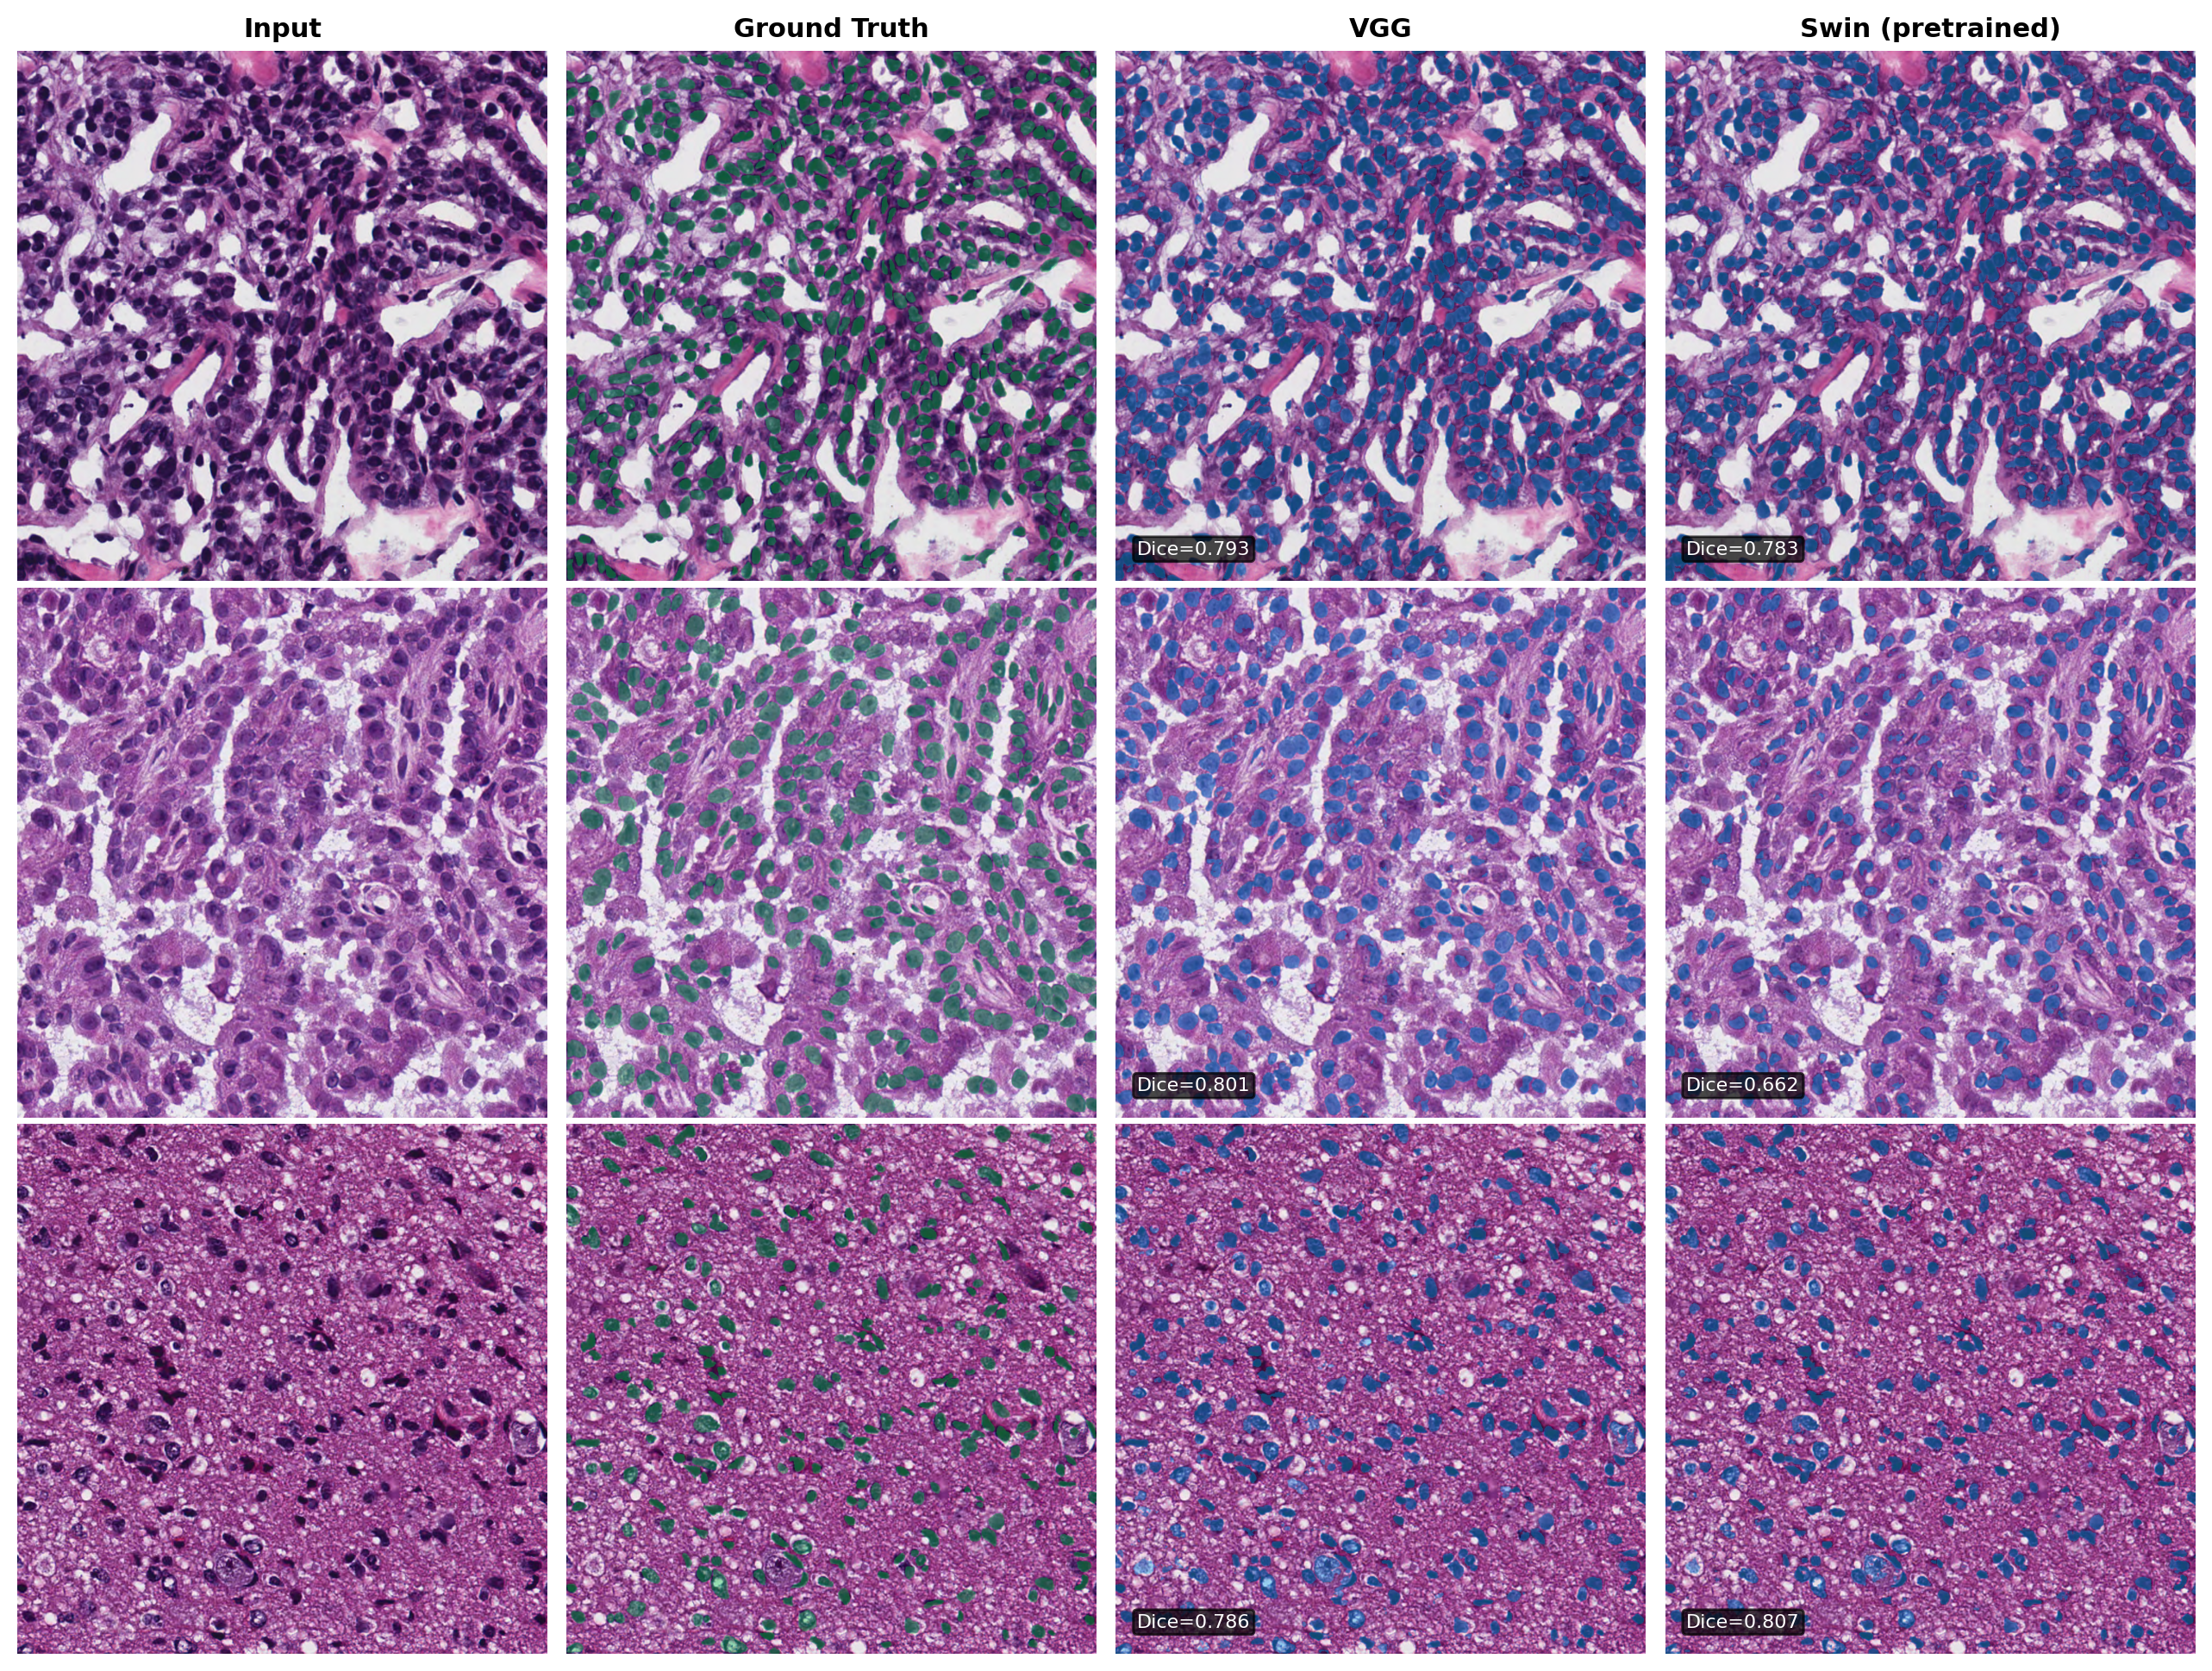
\includegraphics[width=\textwidth]{figures/monuseg_comparison.png}
\caption{Qualitative comparison on three MoNuSeg test images. Columns show the input H\&E patch, ground-truth nucleus overlay (green), VGG prediction (blue), and Swin pretrained prediction (blue). Per-image Dice scores are annotated in each prediction cell. VGG produces tighter boundary delineation; Swin over-segments in dense regions and misses isolated nuclei in sparse regions.}
\label{fig:monuseg_qualitative}
\end{figure}

\subsection{Encoder Comparison: CNN vs.\ Transformer}

Across both datasets, VGG consistently outperforms Swin ($+$0.049 Dice on PanNuke, $+$0.046 on MoNuSeg over pretrained Swin). The from-scratch Swin barely exceeds Otsu on PanNuke (0.590 vs.\ 0.482), confirming that transformers without pretraining lack sufficient inductive bias at this scale. ImageNet pretraining dramatically improves Swin ($+$0.212 Dice) but still fails to close the gap to CNN encoders trained from scratch. The central finding is that CNN inductive biases are competitive with purpose-built small-data transformer architectures, and this advantage is consistent across both data regimes.

\subsection{VGG vs.\ ResNet}

VGG and ResNet produce nearly identical results on PanNuke (0.851 vs.\ 0.849 Dice). This is consistent with the observation that residual connections primarily address the degradation problem in \emph{deep} networks~\cite{he2016resnet}. With only four encoder stages, neither architecture suffers from gradient degradation, and residual shortcuts provide no measurable benefit. We report VGG as the recommended lightweight baseline due to its simpler implementation.

\subsection{Loss Function}

BCE and Dice loss produce virtually identical results (0.851 vs.\ 0.851 Dice; 0.744 vs.\ 0.743 IoU on PanNuke). On datasets where nuclei occupy a reasonable fraction of each patch, BCE does not suffer from class imbalance. Dice loss provides a larger advantage on datasets with very sparse foreground.

\subsection{Training Dynamics}

CNN encoders converge rapidly with stable dynamics; the VGG encoder's step-decay at epoch 30 produces a visible improvement (Dice $0.843 \to 0.848$). The pretrained Swin converges much more slowly and plateaus in the 0.800--0.806 Dice range from epoch 46 onward, while from-scratch Swin shows large oscillations and early-stops with poor performance. Training curves are shown in Appendix~\ref{app:training_curves}.

\subsection{Inference Cost}
\label{sec:inference_cost}

Table~\ref{tab:inference_cost} reports inference-time resource usage on our testbed (Apple~M3, MPS backend), measured as the mean forward-pass latency over 100 iterations on a single $256\times256$ input after a 10-iteration warmup, with peak memory via \texttt{torch.mps.current\_allocated\_memory}. These numbers are reported in support of the lightweight-deployment framing, not as optimized benchmarks (eager-mode PyTorch, no fusion or quantization).

\begin{table}[h]
\centering
\caption{Single-image inference cost at $256\times256$ on Apple~M3 / MPS, batch size~1. Latency is mean over 100 forward passes after warmup. VGG is the fastest and most memory-efficient learned model.}
\label{tab:inference_cost}
\small
\begin{tabular}{@{}lrrr@{}}
\toprule
\textbf{Model} & \textbf{Params} & \textbf{Latency (ms)} & \textbf{Peak Memory (MB)} \\
\midrule
VGG U-Net & 34.0M & 25.2 & 130.5 \\
ResNet U-Net & 37.5M & 34.2 & 144.0 \\
Swin-T U-Net (pretrained) & 86.8M & 46.6 & 333.6 \\
\bottomrule
\end{tabular}
\end{table}

Swin uses roughly $2.6\times$ the memory and $1.8\times$ the latency of VGG for no gain in accuracy. For comparison, pathology foundation models in the 300M--1B parameter range~\cite{chen2024uni, vorontsov2024virchow} require roughly an order of magnitude more memory at inference and are typically deployed via linear probing on cached embeddings~\cite{tizhoosh2025why, campanella2025clinical}. A VGG U-Net fits comfortably within the memory budget of a consumer-grade laptop GPU; even Swin-T, itself one of the smaller vision transformers, already imposes meaningfully larger cost in this regime.

\subsection{Qualitative Analysis}

Qualitative comparisons across all encoder variants on PanNuke fold3 test patches are provided in Appendix~\ref{app:pannuke_qualitative}. All models perform well on isolated, well-separated nuclei but struggle with dense clusters of overlapping nuclei, where binary segmentation cannot resolve individual instances. This motivates approaches like HoVer-Net~\cite{graham2019hovernet} that predict instance-separating distance maps.

The Swin encoder produces noticeably smoother predictions with less precise boundaries, consistent with spatial information loss from $4\times4$ patch tokenization followed by bilinear upsampling. CNN encoders preserve sharper nuclear boundaries, as their features maintain full spatial resolution through the early stages.

%% ============================================================================
\section{Discussion}
%% ============================================================================

\subsection{Implications for Resource-Constrained Deployment}

Our results have direct implications for practitioners outside well-resourced research environments. Foundation models are memory-hungry and, depending on available hardware, may not be executable at all; they are typically restricted to linear probing rather than full fine-tuning~\cite{tizhoosh2025why}. In contrast, VGG U-Net (${\sim}34$M parameters) trains overnight on a single consumer GPU (8GB VRAM), requires no external pretraining data, and achieves competitive performance even with 37 training images. For the specific deployment scenarios motivating this work---edge-deployed microscopy in under-served settings~\cite{salido2025realtime}, veterinary and rare-disease research~\cite{xiao2025review, neal2025artificial}, and non-H\&E staining protocols where foundation model pretraining distributions misalign~\cite{hua2024pathoduet, dejong2025current}---this result is actionable: a VGG encoder, trained from scratch on whatever annotated data is available, reaches published MedT-level performance in the small-data regime and requires no external data or specialized training infrastructure.

\subsection{The Role of Pretraining}

The 0.212 Dice gap between from-scratch (0.590) and pretrained (0.802) Swin on PanNuke is the largest single effect in our experiments and clarifies where the Swin deficit actually lives. Pretraining is not failing---it closes most of the gap from Otsu to CNN performance. What it cannot close is the remaining 0.049 Dice to VGG, which we attribute to the spatial-resolution bottleneck at the skip connections (Section~\ref{sec:intuition}): an architectural property of the encoder, not of its weights. This predicts that domain-matched pretraining (e.g., UNI~\cite{chen2024uni}) would narrow but not close the gap to CNN encoders---a falsifiable claim our budget did not permit testing, and a concrete target for future work.

%% ============================================================================
\section{Conclusion}
%% ============================================================================

We presented a controlled comparison of CNN and transformer encoder architectures for nucleus segmentation in histopathology images, motivated by the deployment gap between large-scale pathology foundation models and the resource constraints of real-world clinical and research settings. Using a U-Net with a fixed decoder and shared encoder interface, evaluated on PanNuke and MoNuSeg, we find that a simple VGG encoder (34M parameters, trained from scratch) outperforms pretrained Swin Transformer on both benchmarks and reaches published MedT-level performance on MoNuSeg (both 0.796 Dice), though with protocol differences (37 vs.\ 30 training images; $256\times256$ patches vs.\ $512\times512$ whole images) that make this a rough equivalence rather than a strict head-to-head. The hypothesized mechanism---spatial resolution preservation at the skip connections combined with convolutional inductive bias---is consistent with the consistent CNN margin across both data scales.

The practical recommendation is clear: for practitioners building nucleus segmentation pipelines with tens of annotated images and single-GPU infrastructure, a VGG U-Net encoder is the strongest available lightweight option. Transformer architectures require either pretraining on large external datasets or substantially more data to match CNN performance, and purpose-built small-data transformers like MedT offer no measurable advantage over a simple VGG encoder at equivalent performance.

\textbf{Future work.} Several directions could extend this study: (1)~evaluation on non-H\&E stained tissue (IHC, fluorescence microscopy) where foundation model pretraining misaligns most severely; (2)~quantifying the training data crossover point at which pretrained Swin begins to match VGG; (3)~hybrid CNN-transformer architectures that use convolutional stems for spatial detail and transformer blocks for global context; and (4)~direct comparison against pathology foundation models (UNI, Virchow2) under memory-matched conditions to characterize the practical tradeoff between model scale and downstream performance.

All code, configurations, and trained checkpoints will be made available to the instructional staff for reproducibility verification.

{\small
\bibliographystyle{plainnat}
\begin{thebibliography}{20}

\bibitem[Wightman(2019)]{rw2019timm}
Ross Wightman.
\newblock PyTorch Image Models.
\newblock \url{https://github.com/huggingface/pytorch-image-models}, 2019.

\bibitem[Ronneberger et~al.(2015)]{ronneberger2015unet}
Olaf Ronneberger, Philipp Fischer, and Thomas Brox.
\newblock U-Net: Convolutional networks for biomedical image segmentation.
\newblock In \emph{MICCAI}, pages 234--241, 2015.

\bibitem[He et~al.(2016)]{he2016resnet}
Kaiming He, Xiangyu Zhang, Shaoqing Ren, and Jian Sun.
\newblock Deep residual learning for image recognition.
\newblock In \emph{CVPR}, pages 770--778, 2016.

\bibitem[He et~al.(2015)]{he2015msra}
Kaiming He, Xiangyu Zhang, Shaoqing Ren, and Jian Sun.
\newblock Delving deep into rectifiers: Surpassing human-level performance on ImageNet classification.
\newblock In \emph{ICCV}, pages 1026--1034, 2015.

\bibitem[Simonyan and Zisserman(2014)]{simonyan2014vgg}
Karen Simonyan and Andrew Zisserman.
\newblock Very deep convolutional networks for large-scale image recognition.
\newblock \emph{arXiv preprint arXiv:1409.1556}, 2014.

\bibitem[Dosovitskiy et~al.(2021)]{dosovitskiy2020vit}
Alexey Dosovitskiy, Lucas Beyer, Alexander Kolesnikov, Dirk Weissenborn, Xiaohua Zhai, Thomas Unterthiner, Mostafa Dehghani, Matthias Minderer, Georg Heigold, Sylvain Gelly, Jakob Uszkoreit, and Neil Houlsby.
\newblock An image is worth 16x16 words: Transformers for image recognition at scale.
\newblock In \emph{ICLR}, 2021.

\bibitem[Liu et~al.(2021)]{liu2021swin}
Ze Liu, Yutong Lin, Yue Cao, Han Hu, Yixuan Wei, Zheng Zhang, Stephen Lin, and Baining Guo.
\newblock Swin Transformer: Hierarchical vision transformer using shifted windows.
\newblock In \emph{ICCV}, pages 10012--10022, 2021.

\bibitem[Ioffe and Szegedy(2015)]{ioffe2015batchnorm}
Sergey Ioffe and Christian Szegedy.
\newblock Batch normalization: Accelerating deep network training by reducing internal covariate shift.
\newblock In \emph{ICML}, pages 448--456, 2015.

\bibitem[Gamper et~al.(2019)]{gamper2019pannuke}
Jevgenij Gamper, Navid~Alemi Koohbanani, Ksenija Benet, Syed~Ali Khuram, and Nasir Rajpoot.
\newblock PanNuke: An open pan-cancer histology dataset for nuclei instance segmentation and classification.
\newblock In \emph{Digital Pathology (ECDP)}, pages 11--19, 2019.

\bibitem[Gamper et~al.(2020)]{gamper2020pannuke_ext}
Jevgenij Gamper, Navid~Alemi Koohbanani, Simon Graham, Mostafa Jahanifar, Syed~Ali Khurram, Ayesha Azam, Katherine Hewitt, and Nasir Rajpoot.
\newblock PanNuke dataset extension, insights and baselines.
\newblock \emph{arXiv preprint arXiv:2003.10778}, 2020.

\bibitem[Kumar et~al.(2017)]{kumar2017monuseg}
Neeraj Kumar, Ruchika Verma, Sanuj Sharma, Surabhi Bhargava, Abhishek Vahadane, and Amit Sethi.
\newblock A dataset and a technique for generalized nuclear segmentation for computational pathology.
\newblock \emph{IEEE Transactions on Medical Imaging}, 36(7):1550--1560, 2017.

\bibitem[Graham et~al.(2019)]{graham2019hovernet}
Simon Graham, Quoc~Dang Vu, Shan~E Ahmed~Raza, Ayesha Azam, Yee~Wah Tsang, Jin~Tae Kwak, and Nasir Rajpoot.
\newblock HoVer-Net: Simultaneous segmentation and classification of nuclei in multi-tissue histology images.
\newblock \emph{Medical Image Analysis}, 58:101563, 2019.

\bibitem[Otsu(1979)]{otsu1979threshold}
Nobuyuki Otsu.
\newblock A threshold selection method from gray-level histograms.
\newblock \emph{IEEE Transactions on Systems, Man, and Cybernetics}, 9(1):62--66, 1979.

\bibitem[Hörst et~al.(2023)]{cellvit2023}
Fabian Hörst, Moritz Rempe, Lukas Heine, et~al.
\newblock CellViT: Vision Transformers for precise cell segmentation and classification.
\newblock \emph{Medical Image Analysis}, 94:103143, 2024.

\bibitem[Baumann et~al.(2024)]{hoverneXt2023}
Elias Baumann, Bettina Dislich, Josef~L. Rumberger, Iris~D. Nagtegaal, Mart{\'\i}nez M.~R., and Inti Zlobec.
\newblock HoVer-NeXt: A fast nuclei segmentation and classification pipeline for next generation histopathology.
\newblock In \emph{Proceedings of the 7th International Conference on Medical Imaging with Deep Learning}, PMLR~250, pages 61--86, 2024.

\bibitem[Valanarasu et~al.(2021)]{valanarasu2021medt}
Jeya~Maria~Jose Valanarasu, Poojan Oza, Ilker Hacihaliloglu, and Vishal~M. Patel.
\newblock Medical Transformer: Gated axial-attention for medical image segmentation.
\newblock In \emph{MICCAI}, pages 36--46, 2021.

\bibitem[Chen et~al.(2024)]{chen2024uni}
Richard~J. Chen, Tong Ding, Ming~Y. Lu, Drew~F.K. Williamson, et~al.
\newblock Towards a general-purpose foundation model for computational pathology.
\newblock \emph{Nature Medicine}, 30(3):850--862, 2024.

\bibitem[Vorontsov et~al.(2024)]{vorontsov2024virchow}
Eugene Vorontsov, Alican Bozkurt, Adam Casson, et~al.
\newblock A foundation model for clinical-grade computational pathology and rare cancers detection.
\newblock \emph{Nature Medicine}, 30(10):2924--2935, 2024.

\bibitem[Campanella et~al.(2025)]{campanella2025clinical}
Gabriele Campanella, Shengjia Chen, et~al.
\newblock A clinical benchmark of public self-supervised pathology foundation models.
\newblock \emph{Nature Communications}, 16:3640, 2025.

\bibitem[Tizhoosh(2025)]{tizhoosh2025why}
Hamid~R. Tizhoosh.
\newblock Why foundation models in pathology are failing.
\newblock \emph{arXiv preprint arXiv:2510.23807}, 2025.

\bibitem[de~Jong et~al.(2025)]{dejong2025current}
Edwin~D. de~Jong, et~al.
\newblock Current pathology foundation models are unrobust to medical center differences.
\newblock \emph{arXiv preprint arXiv:2501.18055}, 2025.

\bibitem[Hua et~al.(2024)]{hua2024pathoduet}
Shengyi Hua, Fang Yan, Tianle Shen, Lei Ma, and Xiaofan Zhang.
\newblock PathoDuet: Foundation models for pathological slide analysis of {H\&E} and {IHC} stains.
\newblock \emph{arXiv preprint arXiv:2312.09894}, 2024.

\bibitem[Bueno et~al.(2025)]{salido2025realtime}
Gloria Bueno, Lorena~S{\'a}nchez-Vargas, Adri{\'a}n~D{\'i}az-Maroto, Jes{\'u}s~Ruiz-Santaquiteria, Marcial Blanco, Jes{\'u}s Salido, and Gabriel Crist{\'o}bal.
\newblock Real-time edge computing vs.\ {GPU}-accelerated pipelines for low-cost microscopy applications.
\newblock \emph{Electronics}, 14(5):930, 2025.

\bibitem[Xiao et~al.(2025)]{xiao2025review}
Sam Xiao, Navneet~K. Dhand, Zhiyong Wang, Kun Hu, Peter~C. Thomson, John~K. House, and Mehar~S. Khatkar.
\newblock Review of applications of deep learning in veterinary diagnostics and animal health.
\newblock \emph{Frontiers in Veterinary Science}, 12:1511522, 2025.

\bibitem[Neal et~al.(2025)]{neal2025artificial}
S.~V. Neal, et~al.
\newblock Artificial intelligence in veterinary clinical pathology---an introduction and review.
\newblock \emph{Veterinary Clinical Pathology}, 2025.

\end{thebibliography}
}

\appendix

\section*{Appendix}

%% ============================================================================
\section{Training Dynamics}
\label{app:training_curves}
%% ============================================================================

\begin{figure}[h]
\centering
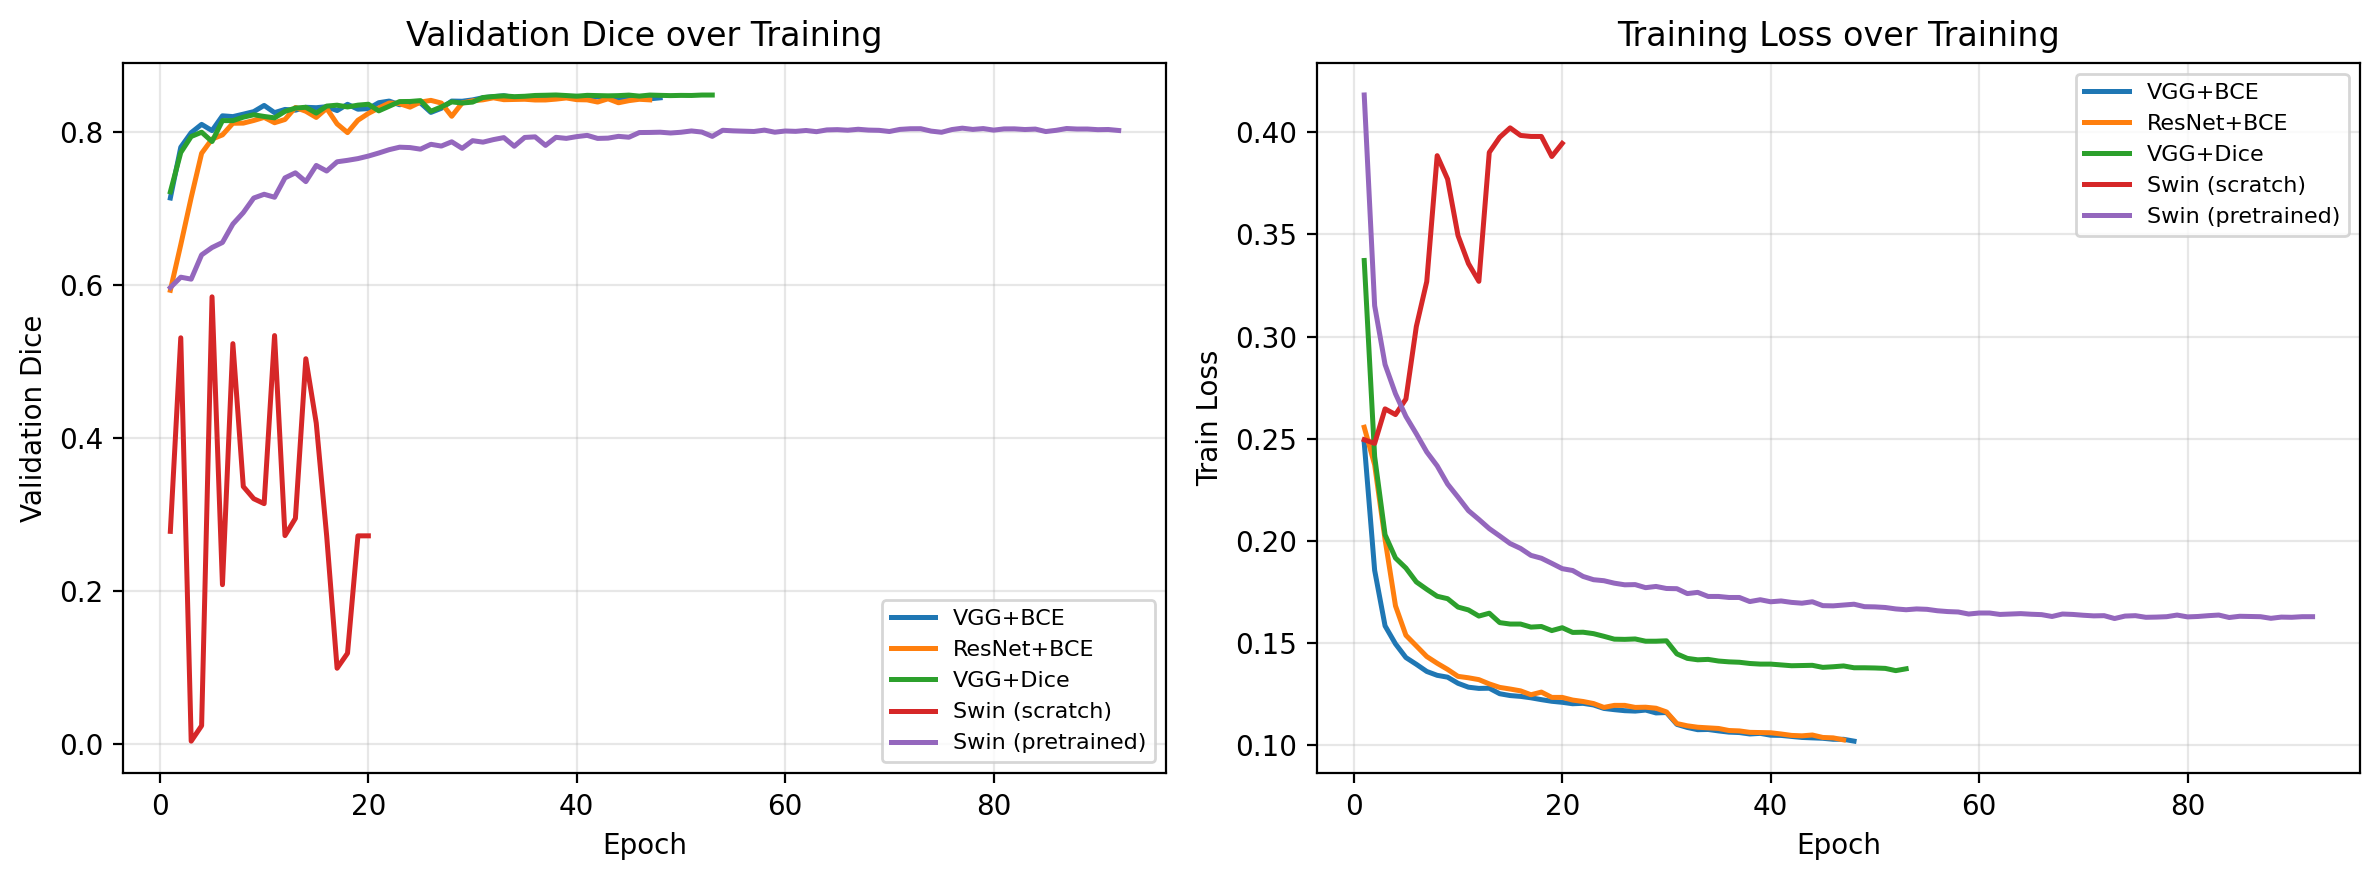
\includegraphics[width=\textwidth]{figures/training_curves.png}
\caption{Validation Dice (left) and training loss (right) over epochs for all encoder variants on PanNuke.}
\label{fig:training_curves}
\end{figure}

%% ============================================================================
\section{PanNuke Qualitative Comparison}
\label{app:pannuke_qualitative}
%% ============================================================================

\begin{figure}[h]
\centering
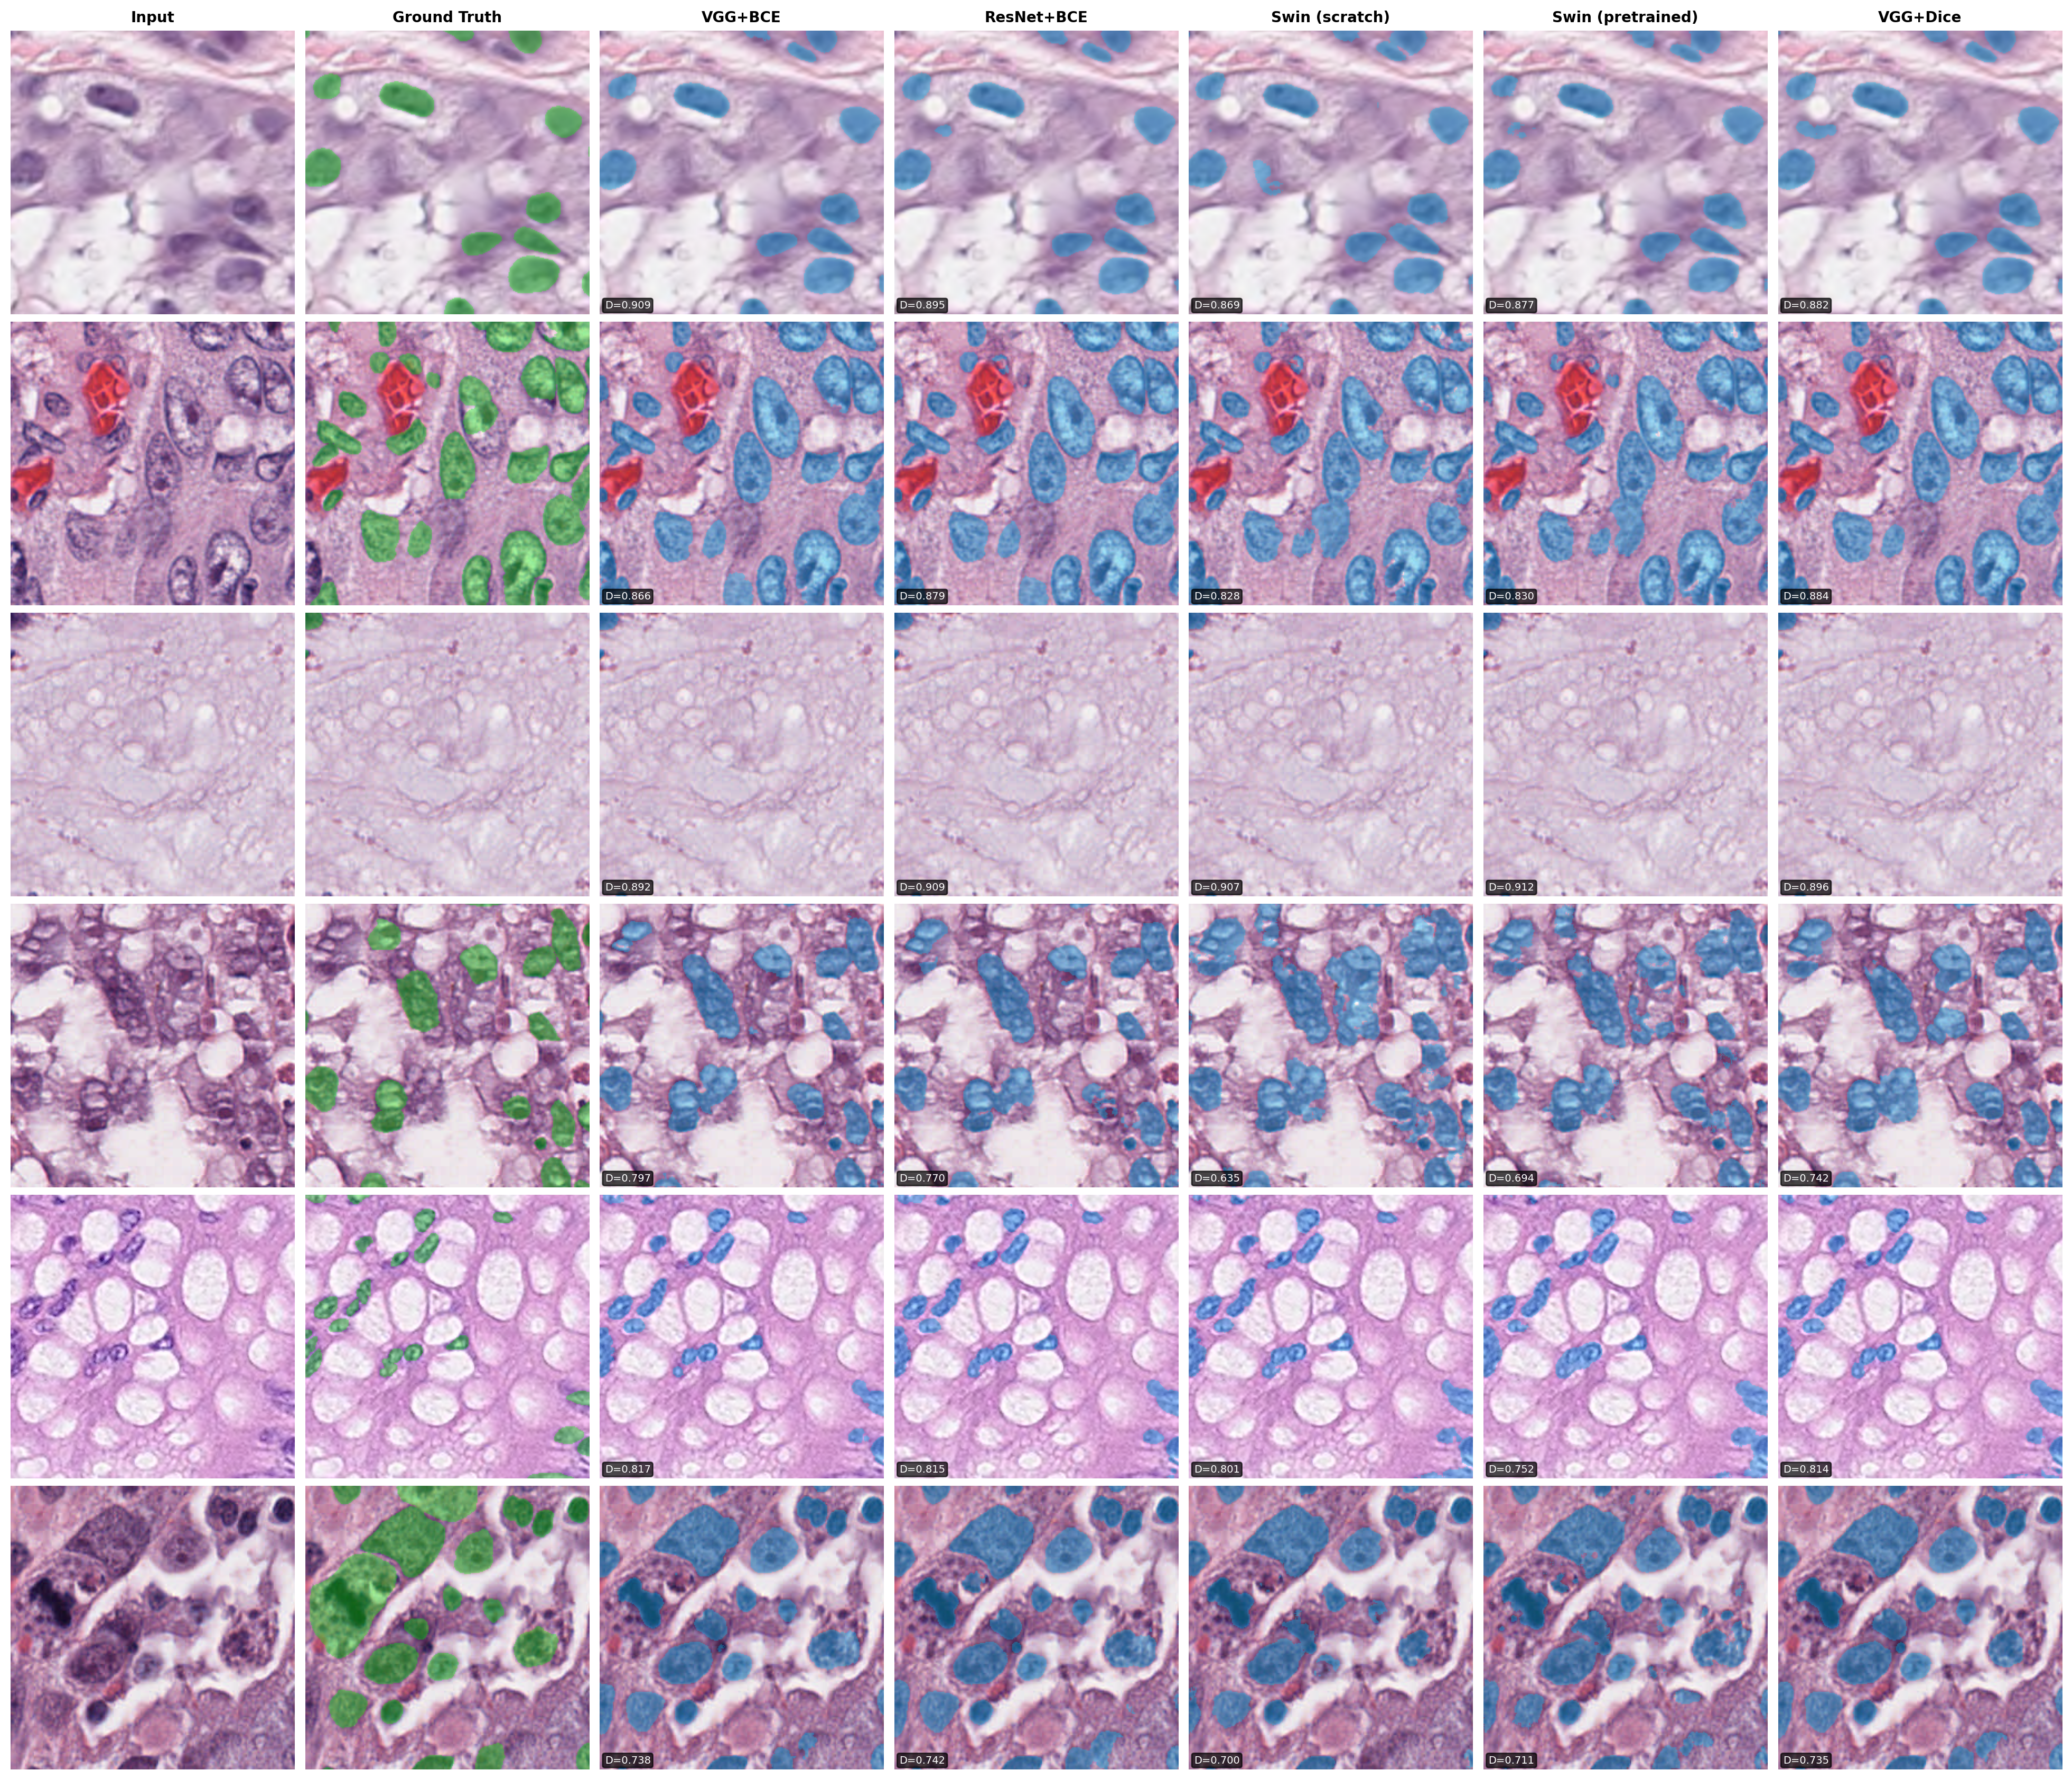
\includegraphics[width=\textwidth]{figures/summary_grid.png}
\caption{Qualitative comparison across models on PanNuke fold3 test patches. Columns (left to right): input H\&E patch, ground-truth overlay, and predictions from VGG+BCE, ResNet+BCE, VGG+Dice, Swin (scratch), and Swin (pretrained). Color coding: green (ground-truth mask in GT column), blue (true positive pixels, i.e., correctly predicted nuclei), red (false negatives, i.e., ground-truth nuclei missed by the model; visible where the model fails to segment a clearly annotated nucleus). Per-sample Dice scores are annotated in each prediction cell.}
\label{fig:qualitative}
\end{figure}

\end{document}